\chapter{\IfLanguageName{dutch}{Stand van zaken}{State of the art}}%
\label{ch:stand-van-zaken}
%todo sectie over verduidelijking termen, zoals design pattern, architectuur, energieefficiëntie, ...
\section{Inleiding}
Todo: overal een kort inleidende paragraaf, dit wordt pas gedaan eenmaal de sectie af is om een volledig beeld te schetsen hoe het past in de bachelorproef.\\
In deze sectie ben ik van plan enkele termen al te verduidelijken om het vervolg van de literatuurstudie duidelijker te maken.


\section{Ontwikkelarchitecturen}
%TODO inleidende paragraaf
Inleidende paragraaf:

\subsection{Wat is een architectuur}
Een softwareontwikkelarchitectuur is een infrastructuur waarin applicatie componenten, die de functionele requirements voorzien, gespecificeerd, geïmplementeerd en uitgevoerd kunnen worden \autocite{Solms2012}. 

\subsection{Nut van architectuur}
\textcite{Jaiswal2019} stelt dat een architectuur de blauwdruk is van een systeem, waarbij het complexiteit beheert en communicatie tussen componenten mogelijk maakt. Het levert een gestructureerde oplossing voor technische en operationele eisen, met aandacht voor kwaliteitskenmerken zoals prestaties en beveiliging. De keuze van architectuur is een belangrijke beslissing die een aanzienlijke invloed heeft op de kwaliteit en het succes van het eindproduct.


\subsection{Opbouw architectuur}
Volgens \textcite{Solms2012} is een softwarearchitectuur opgebouwd uit 4 elementen:
\begin{itemize}
    \item Basis concepten en regels voor applicatie componenten die gebruikersfunctionaliteit voorzien;
    \item Architecturale componenten die technische zaken aanpakken;
    \item Manieren waarop er intern en/of extern met de applicatie gecommuniceerd wordt;
    \item Architecturale strategieën die de software kwaliteit beïnvloeden.
\end{itemize}


De basis concepten en regels zijn specifiek voor de bepaalde architectuur. Ze hebben 2 specifieke doelen, namelijk als extra documentatie om de architectuur beter te begrijpen en later makkelijk uitbreidingen toe te laten en te verifiëren of ze voldoen aan vooraf opgestelde regels en pricipes \autocite{Oussalah2013}. Verder hebben ze invloed op zowel de designfase als de implementatiefase.\\

Architecturale componenten worden onderverdeeld in gebruikersinterface en structurele componenten \autocite{EDUCBA2023}. Zaken zoals de functionaliteiten van de client en server, maar ook de database interactie worden behandeld door de structurele componenten. Verder kan er ook onderverdeeld worden in verschillende lagen, zoals in figuur \ref{architectural_components_sota}. Hierin wordt de architectuur van een applicatie, iEnvironment, getoond. Er is de externe toegangslaag voor gebruikers die verbonden is met de gebruikersinterface laag. Die gaat dan op zijn beurt connectie maken naar de applicatielaag, datalaag en eventueel een externe toegangslaag waar data opgeslagen wordt. Elk van deze lagen is verantwoordelijk voor een bepaalde functionaliteit en zijn noodzakelijk om de volledige applicatie correct te laten verlopen.

\begin{figure}[ht]
    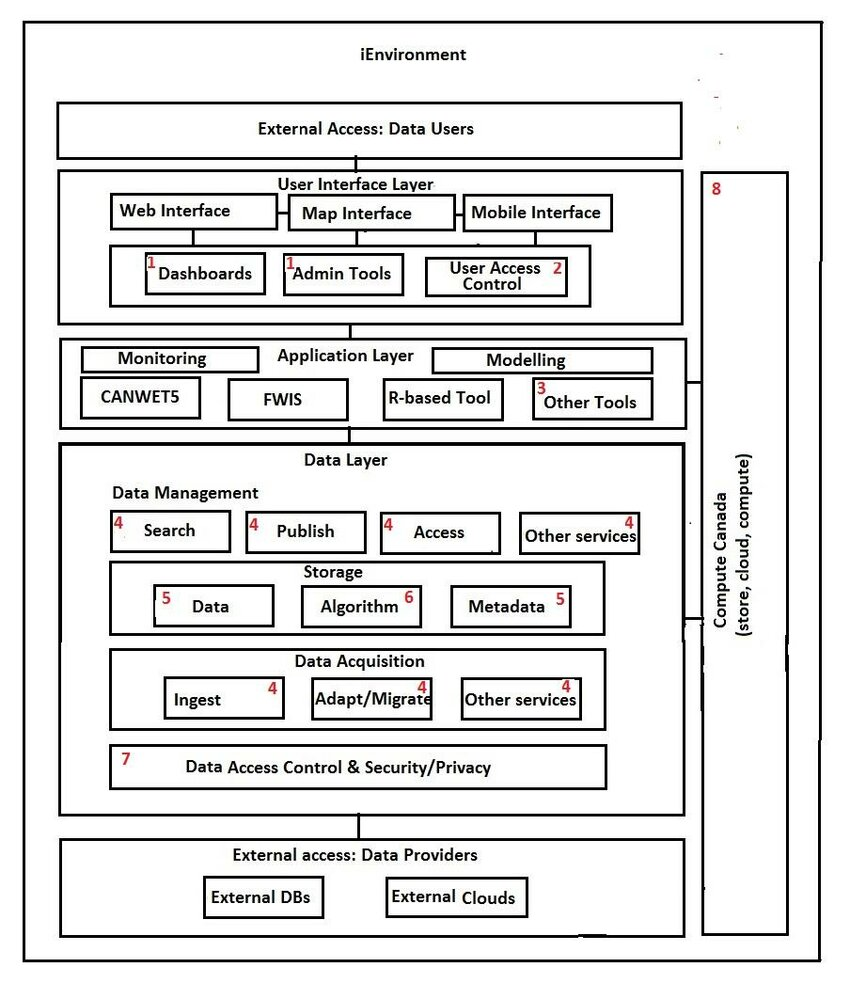
\includegraphics[scale=0.5]{architectural_components_sota}
    \centering
    \caption{Architecturale componenten iEnvironment \autocite{Alencar2018}}
    \label{architectural_components_sota}
\end{figure}

\bigskip

De manieren waarop er gecommuniceerd kan worden met de applicatie moet ook duidelijk aangegeven zijn in de architectuur. Zo wordt de toegang en integratie gespecificeerd voor functionaliteit binnen de architectuur, applicatie logica voor externe functionaliteiten en tussen de architecturale componenten van de architectuur. Zo kan er bijvoorbeeld een web gebaseerde interface zijn voor menselijke gebruikers, terwijl systemen gebruik kunnen maken van web services zoals API's.\\

Als laatste zijn er de architecturale strategieën of ook wel tactieken genoemd. Ze zijn  ontwerpbeslissingen die het antwoord van de applicatie op een specifieke actie beïnvloeden dat belangrijk is voor bepaalde QA, quality attributes \autocite{Marquez2023}. Enkele QA die beïnvloedt kunnen worden door deze tactieken zijn aanpasbaarheid, afhankelijkheid, betrouwbaarheid, performantie, schaalbaarheid, ...

\subsection{Verschillende architecturen}
\subsubsection{Monolithisch}
Alhoewel nog vaak voorkomend is de monolithische architectuur eerder verouderd waar geen gebruik gemaakt wordt van modulariteit \autocite{Megargel2020}. De user interface werd direct verbonden met business logica die doorverbonden stond met een database, zoals voorgesteld in figuur \ref{monolith_sota}. Elk onderdeel wordt gedefinieerd als een distinctieve architectuurlaag van een monoliet applicatie, respectievelijk de user interfacelaag, business logicalaag en databaselaag. \\

\begin{figure}[H]
    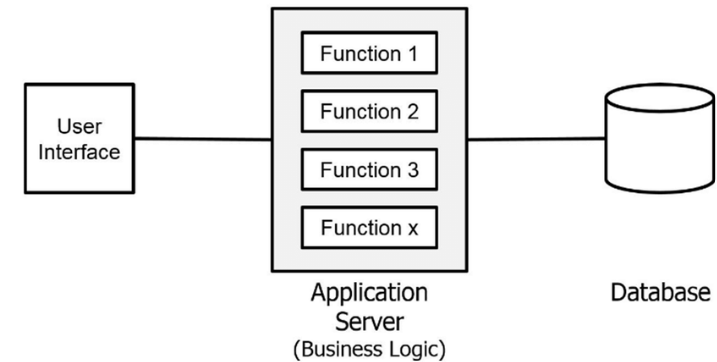
\includegraphics[scale=0.8]{monolith_sota}
    \centering
    \caption{Voorstelling monoliet \autocite{Megargel2020}}
    \label{monolith_sota}
\end{figure}


Het basis concept van deze architectuur is het centraal verzamelen van alle functies. Zoals vermeld zijn de architecturale componenten bij een monolithische architectuur duidelijk aanwezig. Echter zorgt deze structuur ervoor dat schaalbaarheid heel moeilijk verwezenlijkt kan worden. Het overbelasten van 1 functie zal veel resources in beslag nemen, die door alle functies gebruikt moet worden. Het verticaal schalen is hier de oplossing voor, met het toevoegen van meer RAM bijvoorbeeld, maar is niet altijd een haalbare oplossing. Aangezien alle modules of functies van de applicatie op 1 server gedeployed zijn gebeurd alle communicatie binnen hetzelfde proces en is er geen netwerk communicatie nodig \autocite{Ozkaya2023}. 


\subsubsection{Microservices}
Microservices zijn een variant van de service-georiënteerde architectuur. Het bestaat uit een verzameling van kleine losse services die samenwerken tot de werking van een volledige applicatie \autocite{Megargel2020}. Een microservice omvat een business entiteit, bijvoorbeeld een product of een klant, of kan bepaalde activiteiten omvatten, zoals het plaatsen van een bestelling bij een webshop. Dit wordt visueel weergegeven in figuur \ref{microservice_sota} waar elk bolletje een microservice voorstelt die op zijn beurt een bepaalde functionaliteit van een business entiteit afhandelt.\\

\begin{figure}[H]
    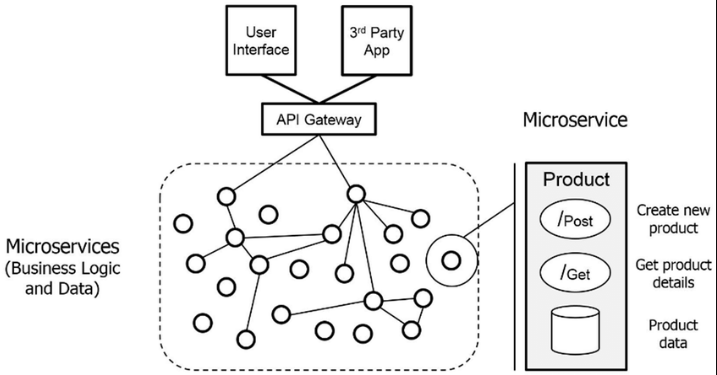
\includegraphics{microservice_sota}
    \caption{Voorstelling microservice architectuur \autocite{Megargel2020}}
    \label{microservice_sota}
\end{figure}

Het basisconcept bij deze architectuur is om elke functionaliteit zodanig op te splitsen dat elke business entiteit onafhankelijk kan functioneren. De architecturale componenten zijn hier, zoals voorgesteld in figuur \ref{microservice_sota}, een user interface of een applicatie van derden die verbonden is met een verzameling van microservices. De communicatie gebeurt via een API, waardoor zowel web applicaties als andere systemen gebruik kunnen maken van de beschikbaar gestelde functionaliteiten die de microservices bieden. Strategieën die gebruikt kunnen worden bij deze architectuur zijn het deployen naar een cloud omgeving waar alles automatisch geschaald kan worden. Wanneer één service meer belast wordt dan de andere, krijgt deze automatisch meer resources toegewezen zonder dat de andere services beïnvloedt worden. Ook zorgt dit ervoor dat de applicatie grotendeels blijft werken wanneer een microservice (tijdelijk) niet beschikbaar is.

\subsubsection{Gelaagde architectuur}
Todo: Uitleggen van gelaagde architectuur

\subsubsection{Andere architecturen}


\subsection{Samengevat}
Kort kan dus gezegd worden dat een ontwikkelarchitectuur richtlijnen geeft hoe een applicatie ontwikkeld wordt. Het levert een structuur die de prestaties en beveiliging beïnvloeden. De 4 bouwdelen van een architectuur zorgen ervoor dat een applicatie gemakkelijk uitbreidbaar is, logisch is opgebouwd, bereikbaar is zowel voor mens als systemen en voldoet aan kwaliteitseisen.



\section{Energie-efficiëntie}
%todo inleidende paragraaf
Inleidende paragraaf: 

\subsection{Wat is energie-efficiëntie}
 % oud artikel, maar wel interessant!
Energie-efficiëntie is een generieke, niet-meetbare term \autocite{Patterson1996}. Het is wel een vergelijkbare term, in die zin dat er vergeleken wordt hoeveel energie er gebruikt wordt voor eenzelfde service of bruikbare output te verkrijgen in verschillende situaties. Het wordt vaak gedefinieerd als de ratio 
$\frac{\text{Bruikbare output}}{\text{Energie input}}$ .



\subsection{Energieverbruik van software}
%inleiding? Eerdere onderzoeken aanhalen en in subsecties onderverdelen en bespreken.
%todo: hoe wordt precies energie verbruikt door software?
\subsection{Link met programmeertalen}
\autocite{Manner2022}

%verschil compiled, interpreted en 
Volgens \textcite{Jain2024} kan software in 2 manieren verdeeld worden waarop een applicatie vertaalt wordt naar machine taal. Er is compiled language en interpreted language. Compiled gaat de volledige code voor het opstarten van het programma in zijn geheel compileren. Dit leidt tot een efficiëntere applicatie omdat de vertaling van code naar machine taal al gebeurd is. Dit in tegenstelling tot interpreted language. Hier wordt code lijn per lijn vertaald en uitgevoerd. Dit zorgt er dan voor dat de applicatie flexibeler is waardoor het programma minder snel uitgevoerd wordt.\\

Zo blijkt ook uit onderzoek van \textcite{Pereira2017} dat de keuze van programmeertaal een grote impact kan hebben op het energieverbruik van de applicatie. Zo blijkt uit figuur \ref{verbruik_taal_sota} dat C\footnote{https://www.cprogramming.com/}, een compiled language, de meest energiezuinige taal is en Perl\footnote{https://www.perl.org/}, een interpreted taal, het meeste energie verbruikt, namelijk tot wel 80 keer zoveel als C voor het runnen van eenzelfde applicatie. \\

\begin{figure}[H]
    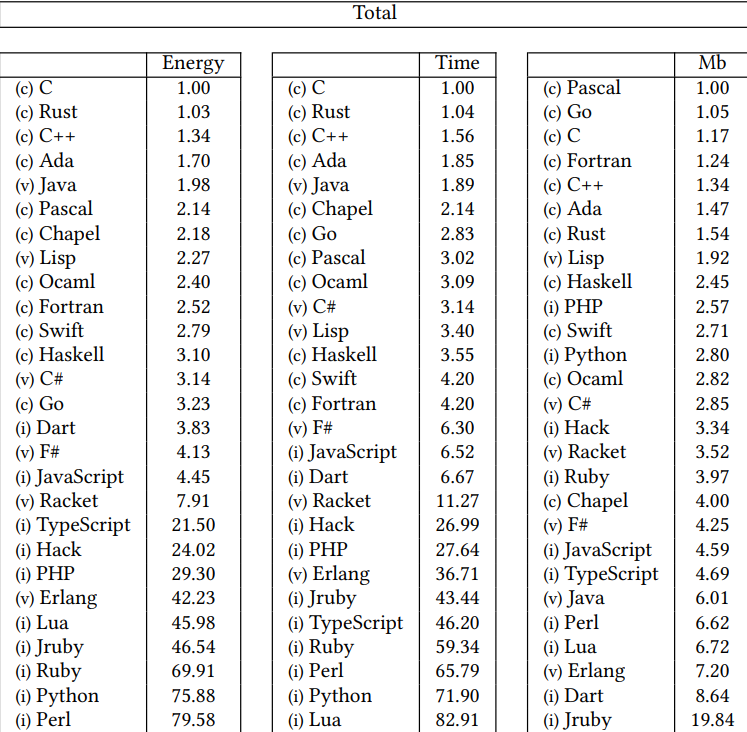
\includegraphics[scale=0.5]{verbruik_taal_sota}
    \centering
    \caption{Genormaliseerd energieverbruik, uitvoeringstijd en geheugengebruik van 1 scenario \autocite{Pereira2017}}
    
    \label{verbruik_taal_sota}
\end{figure}


\subsection{Link met programmeerprincipes}
Bij het ontwikkelen van programma's is de eindfunctionaliteit vaak vastgelegd. Het programma moet namelijk een of meerdere taken kunnen uitvoeren. Echter is het zo dat het niet vastligt hoe het ontwikkeld wordt. Om één bepaalde uitkomst te bekomen zijn er meerdere manieren om dit te verwezenlijken. Wanneer 1 verwachte uitkomst door verschillende programmeurs ontwikkeld wordt, zal er zelden 100\% gelijke code geschreven worden. Dit komt door de eigen stijl/manier van ontwikkelen.

\bigskip

In het onderzoek van \textcite{Hassan2017} wordt aangetoond dat een verschillende programmeerstijl impact kan hebben op het energieverbruik van een applicatie. Zo is er in figuur \ref{3_coding_styles_sota} een selection sort geprogrammeerd op 3 manieren. De eerste manier sorteert eerst de array en zal eenmaal gesorteerd de array uitschrijven naar de console. In de tweede manier wordt tijdens het sorteren al uitgeschreven naar de console en als laatste manier wordt er zoals de eerste stijl gewerkt, maar wordt er om de 500 items een pauze gehouden om de processor even te stoppen en na te gaan of een sleep operatie een invloed heeft op energieverbruik. De resultaten zijn beschikbaar in figuur \ref{energy_consumption_situations_sota}. Hieruit kan er besloten worden dat elke manier verschilt in energieverbruik. Dit is echter niet het enige wat deze resultaten aanduiden. De compilers waarop deze testen uitgevoerd werden hebben duidelijk ook een impact op het energieverbruik.\\

\bigskip

\begin{figure}[H]
    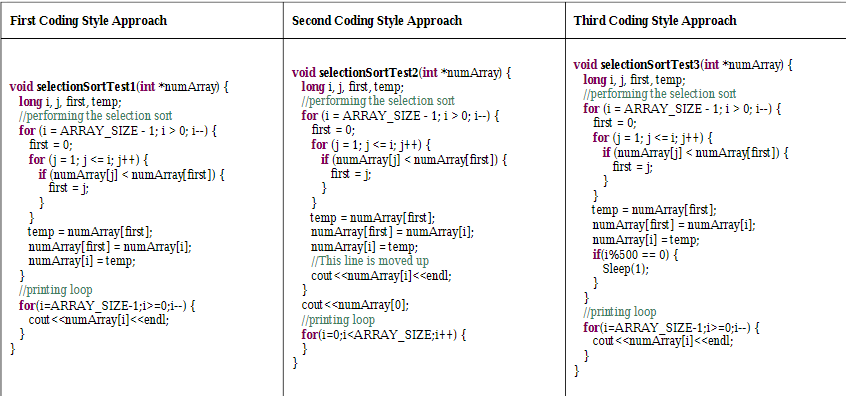
\includegraphics[scale=0.8]{3_coding_styles_sota}
    \centering
    \caption{3 manieren voor een selection sort \autocite{Hassan2017}}
    \label{3_coding_styles_sota}
\end{figure}

\begin{figure}[H]
    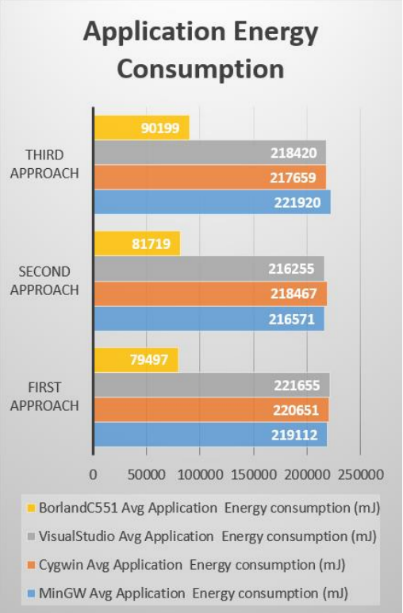
\includegraphics[scale=0.8]{energy_consumption_situations_sota}
    \centering
    \caption[Energieverbruik tussen programmeerstijlen]{Energieverbruik tussen verschillende programmeerstijlen in verschillende compilers \autocite{Hassan2017}}
    \label{energy_consumption_situations_sota}
\end{figure}



Ook datatypes spelen een rol in het energieverbruik van software. Gegevens opslaan in een datatype dat meer plaats inneemt in het geheugen of extra processing power nodig heeft leidt tot een hoger energieverbruik \autocite{Dutta2023}. Zo wordt in figuur \ref{energy_consumption_data_types_sota}, waar numerieke datatypes vergeleken worden, aangetoond dat er tot net geen 50\% energie bespaart kan worden op basis van het datatype. Deze situatie is niet altijd haalbaar, aangezien niet elk van deze datatypes geschikt is voor eenzelfde use case. 

\bigskip

Wat echter wel altijd haalbaar is, is wanneer een string voorgesteld moet worden. Het gebruik maken van een StringBuilder, een ingebouwde klasse die string operaties kan uitvoeren, verbruikt nagenoeg geen energie. Wanneer de gewone String klasse gebruikt wordt, verbruikt dit duizenden keren meer energie dan de StringBuilder. Dit fenomeen wordt aangetoond in figuur \ref{energy_consumption_string_sota}. 

\bigskip


\begin{figure}[H]
    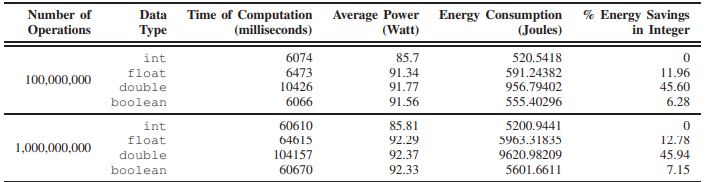
\includegraphics{energy_consumption_data_types_sota}
    \caption[Energieverbruik numerieke datatypes]{Vergelijken van energieverbruik bij numerieke datatypes \autocite{Dutta2023}}
    \label{energy_consumption_data_types_sota}
\end{figure}


\begin{figure}[H]
    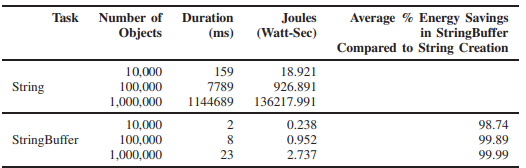
\includegraphics{energy_consumption_string_sota}
    \centering
    \caption[Energieverbruik string voorstelling]{Vergelijken van energieverbruik bij voorstellen van string values \autocite{Dutta2023}}
    \label{energy_consumption_string_sota}

\end{figure}


\subsection{Link met performantie}
Volgens \textcite{Lubomski2020} zijn de 3 karakteristieken die performantie bepalen responstijd, doorvoer van data en gebruik van resources. Ze beïnvloeden elkaar, bijvoorbeeld een trage doorvoer van data leidt tot een lage responstijd. Een performante applicatie probeert te streven naar de beste combinatie van de 3. Dit is dan een hoge datadoorvoer met een laag resource gebruik en een lage responstijd. 

\bigskip

De karakteristiek dat inspeelt op energieverbruik van software is het resource gebruik. Hieronder valt CPU-, RAM-, disk- en netwerkgebruik. Dit wordt bevestigd door figuur \ref{cpu_usage_sota}, waar een hoger CPU-gebruik gelijk staat aan een hoger energieverbruik.\\


%\autocite{Hassan2017} %goed onderzoek

\begin{figure}[h!]
    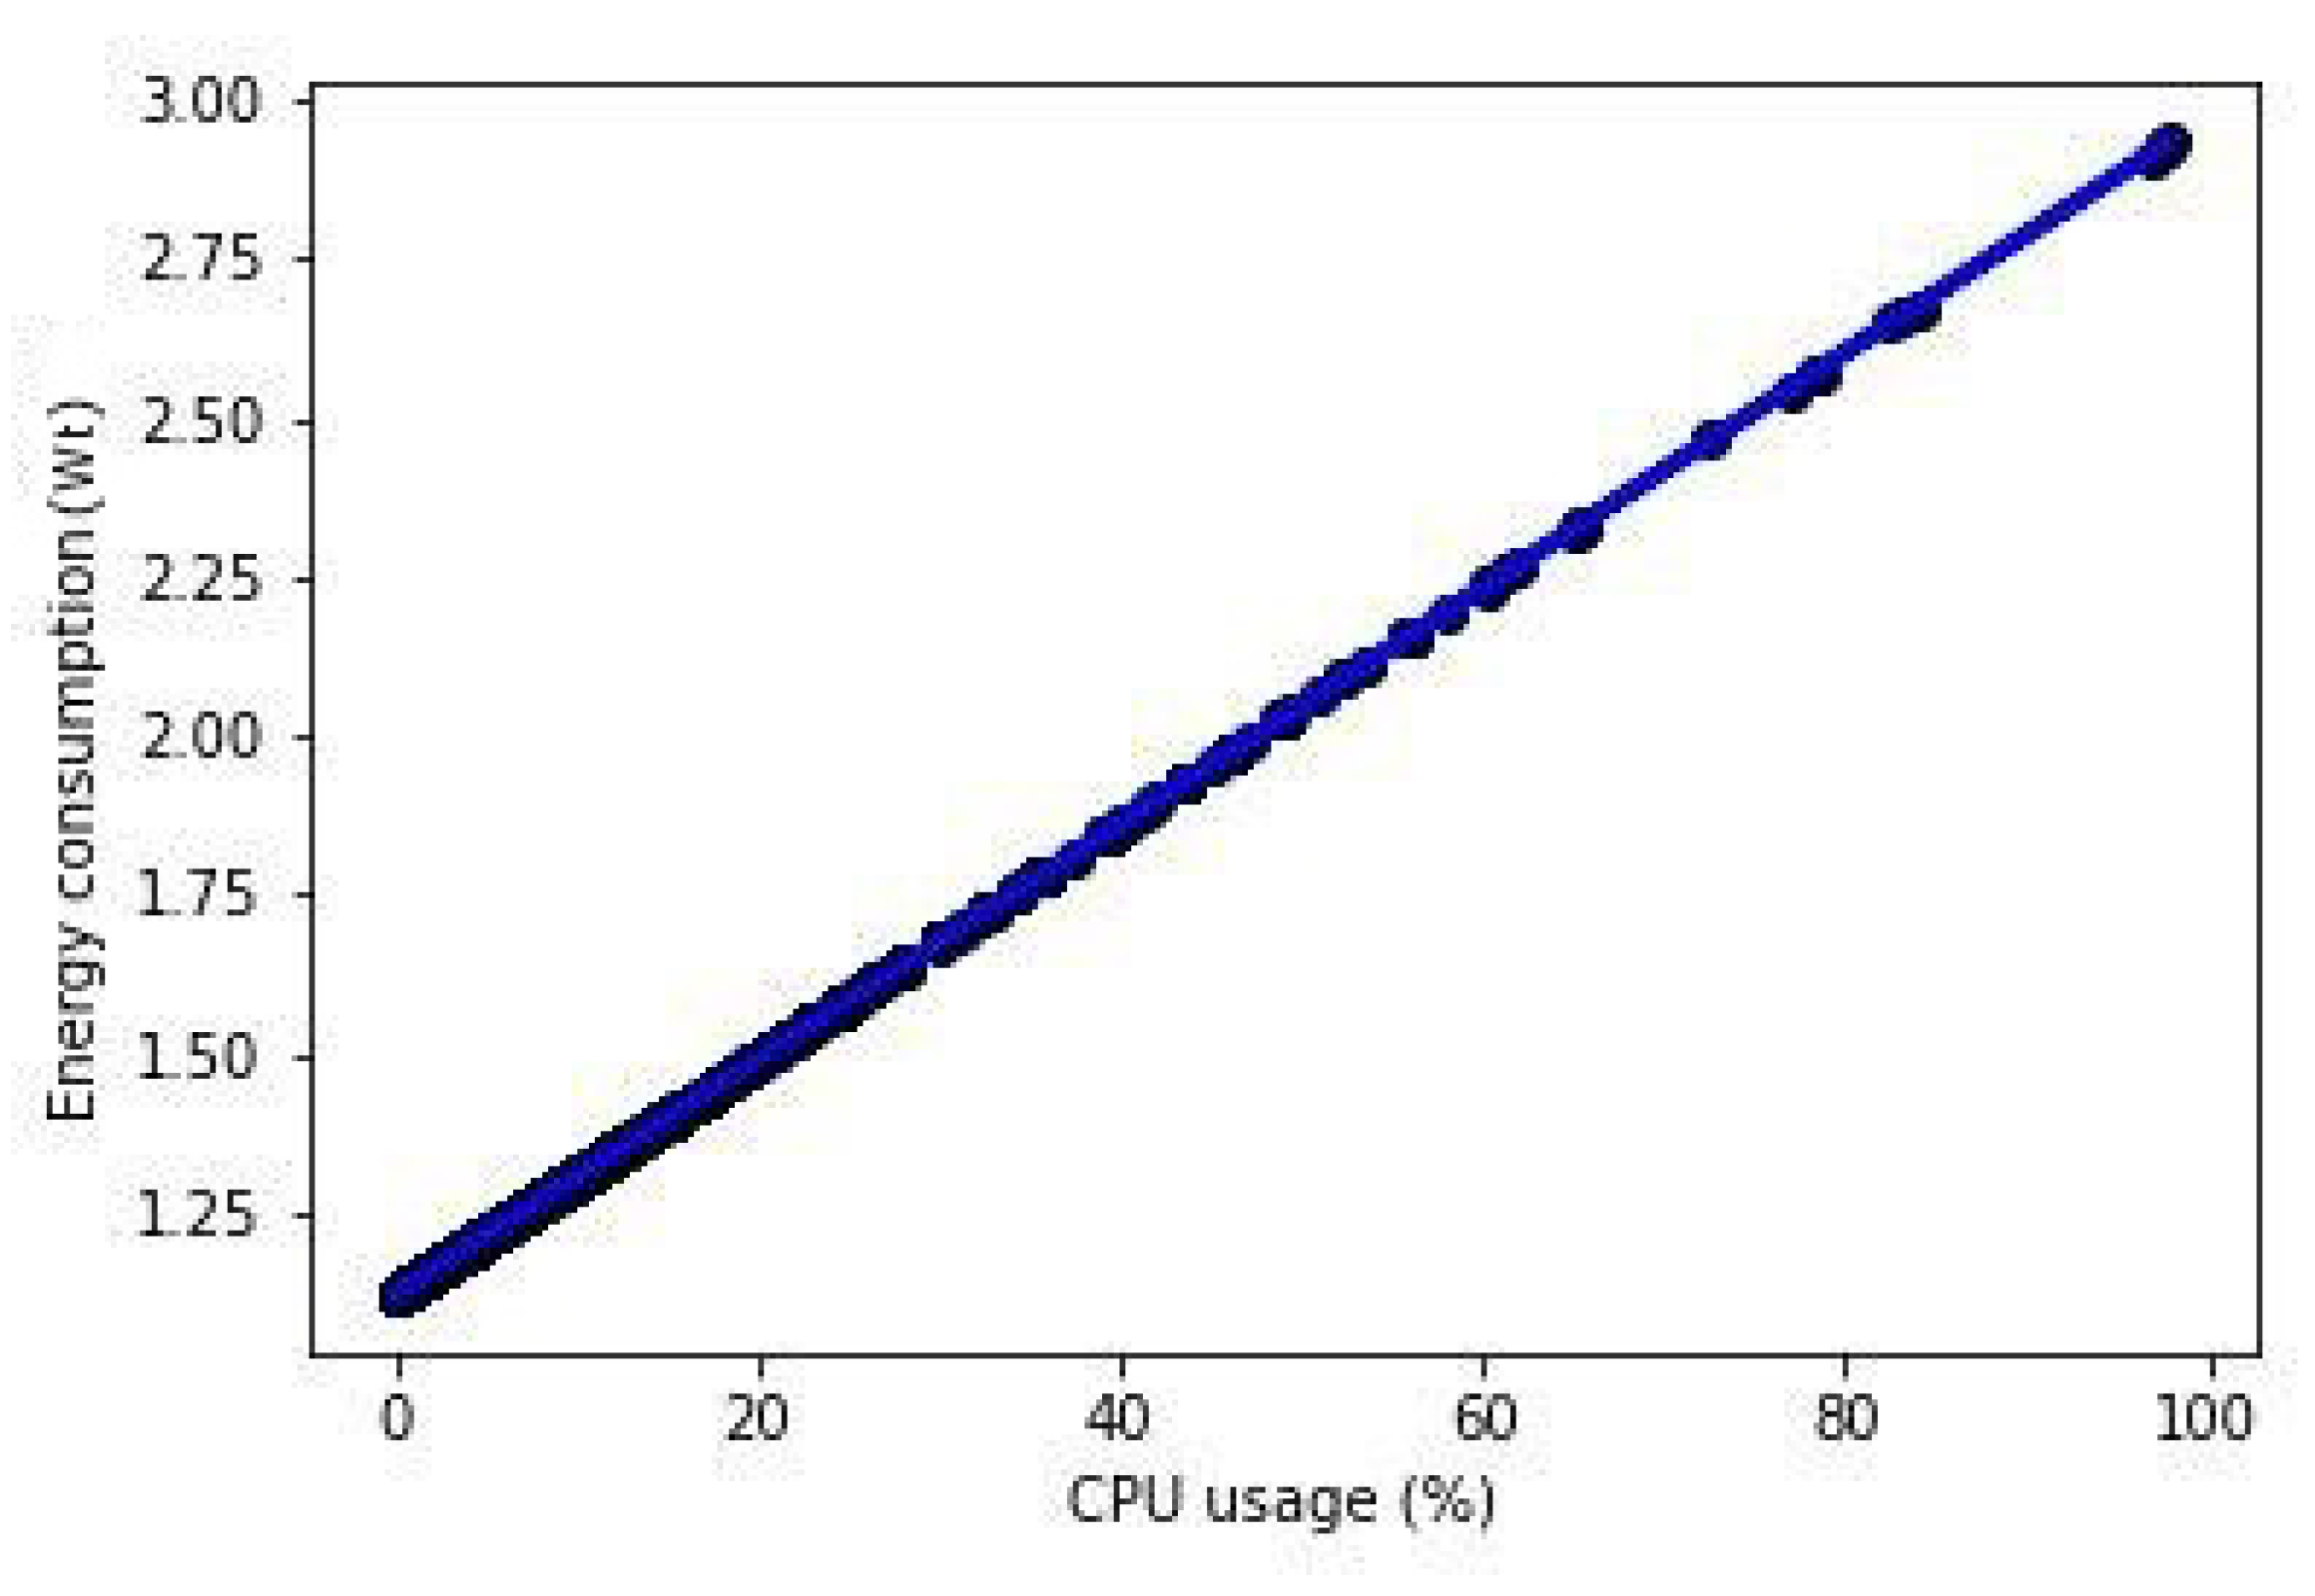
\includegraphics{cpu_usage_sota}
    \centering
    \caption{Representatie verbruik energie (Watt) tegenover CPU-gebruik (\%) \autocite{Ciancarini2020}}
    \label{cpu_usage_sota}
\end{figure}

\subsection{Meten van energieverbruik}
%\autocite{Ergasheva2020} %kan interessant zijn
Het meten van energieverbruik bij software is een complexe taak. Volgens het onderzoek van \autocite{Dutta2023} is het echter niet de software dat energie verbruikt, maar is het de logica van de gecompileerde code die de hardware componenten, zoals de processor en geheugen, aanstuurt die op hun beurt energie verbruiken. Daarom wordt vaak bij het vermelden van `energieverbruik van software` gerefereerd naar het energieverbruik van de hardware componenten die aangestuurd worden door de code.

\bigskip
%todo: paragraaf over het meten van energieverbruik bij software
Twee vaak gebruikte manieren om het energieverbruik te meten van software zijn het gebruik van een energiemeter of een combinatie van processen op een Linux systeem die toelaten om het verbruik softwarematig te meten en visueel voor te stellen in een Grafana\footnote{https://grafana.com/} dashboard. Voor andere operating systems blijkt het niet of moeilijk haalbaar om softwarematig energieverbruik te meten van applicaties. \bigskip

Het meten via een energiemeter heeft als nadeel dat je niet op applicatie- of procesniveau kunt monitoren. Het meet namelijk de stroom dat direct uit het stopcontact verbruikt wordt. Hiermee kan dus wel het totale verbruik van het systeem gemonitord worden. Voor het meten op applicatieniveau kan er eerst een meting gebeuren op een idle systeem, waar het programma niet aan het runnen is, en dan een meting wanneer de applicatie wel actief is. Het verschil is dan het energieverbruik op applicatieniveau, alhoewel dit niet nauwkeurig is omdat eventuele andere achtergrondprocessen geactiveerd of gedeactiveerd kunnen worden tijdens de meting. \bigskip

Het softwarematig meten van energieverbruik laat wel toe om op applicatie- of procesniveau te monitoren. Hiervoor is er een applicatie of proces nodig dat toegang heeft tot alle actieve processen op het systeem, alsook het resourcegebruik hiervan. Afhankelijk van de hardware kan er al dan niet rechtstreeks ook het energieverbruik getoond worden. \bigskip
%https://medium.com/@dreams-smoke/how-to-monitor-power-usage-of-your-linux-computing-system-with-prometheus-grafana-f21b9933762

%\autocite{Procaccianti2015}

\subsection{Samengevat}
Energieverbruik van software is op meerdere vlakken al grondig onderzocht. Zo is er een verschil bij de keuze in programmeertaal. Kiezen voor de meest efficiënte compiled language kan tot wel 80 keer zo energiezuiniger werken dan de minst efficiënte interpreted language. Ook het hanteren van bepaalde programmeerprincipes zoals stijl of datatypes beïnvloeden het energieverbruik. Ook wijzen onderzoeken uit dat de compiler die de code uitvoert een degelijke impact heeft. Verder is performantie ook een belangrijke factor. Inefficiënt gebruik van resources leidt tot hoger energieverbruik van componenten zoals CPU, RAM, disk, ... Om het verbruik van software in kaart te brengen kan er gebruik gemaakt worden van een energiemeter of bepaalde software. Een energiemeter zal minder nauwkeurige resultaten afleveren dan de softwarematige metingen, maar kan in elke situatie gebruikt worden terwijl de softwarematige metingen vaak beperkt zijn tot 1 operating system. 

\section{Literatuurstudie samengevat}
%todo: korte samenvatting wat belangrijk is om te weten uit de literatuurstudie


% Tip: Begin elk hoofdstuk met een paragraaf inleiding die beschrijft hoe
% dit hoofdstuk past binnen het geheel van de bachelorproef. Geef in het
% bijzonder aan wat de link is met het vorige en volgende hoofdstuk.

% Pas na deze inleidende paragraaf komt de eerste sectiehoofding.

%Dit hoofdstuk bevat je literatuurstudie. De inhoud gaat verder op de inleiding, maar zal het onderwerp van de bachelorproef *diepgaand* uitspitten. De bedoeling is dat de lezer na lezing van dit hoofdstuk helemaal op de hoogte is van de huidige stand van zaken (state-of-the-art) in het onderzoeksdomein. Iemand die niet vertrouwd is met het onderwerp, weet nu voldoende om de rest van het verhaal te kunnen volgen, zonder dat die er nog andere informatie moet over opzoeken \autocite{Pollefliet2011}.

%Je verwijst bij elke bewering die je doet, vakterm die je introduceert, enz.\ naar je bronnen. In \LaTeX{} kan dat met het commando \texttt{$\backslash${textcite\{\}}} of \texttt{$\backslash${autocite\{\}}}. Als argument van het commando geef je de ``sleutel'' van een ``record'' in een bibliografische databank in het Bib\LaTeX{}-formaat (een tekstbestand). Als je expliciet naar de auteur verwijst in de zin (narratieve referentie), gebruik je \texttt{$\backslash${}textcite\{\}}. Soms is de auteursnaam niet expliciet een onderdeel van de zin, dan gebruik je \texttt{$\backslash${}autocite\{\}} (referentie tussen haakjes). Dit gebruik je bv.~bij een citaat, of om in het bijschrift van een overgenomen afbeelding, broncode, tabel, enz. te verwijzen naar de bron. In de volgende paragraaf een voorbeeld van elk.

%\textcite{Knuth1998} schreef een van de standaardwerken over sorteer- en zoekalgoritmen. Experten zijn het erover eens dat cloud computing een interessante opportuniteit vormen, zowel voor gebruikers als voor dienstverleners op vlak van informatietechnologie~\autocite{Creeger2009}.

%Let er ook op: het \texttt{cite}-commando voor de punt, dus binnen de zin. Je verwijst meteen naar een bron in de eerste zin die erop gebaseerd is, dus niet pas op het einde van een paragraaf.

%\lipsum[7-20]
